\documentclass[a4paper,11pt]{article}
\usepackage{nopageno} % visto che in questo caso abbiamo una pagina sola
\usepackage{lmodern}
\renewcommand*\familydefault{\sfdefault}
\usepackage{sfmath}
\usepackage[utf8]{inputenc}
\usepackage[T1]{fontenc}
\usepackage[italian]{babel}
\usepackage{indentfirst}
\usepackage{graphicx}
\usepackage{animate}
\usepackage{tikz}
\usepackage{wrapfig}
\newcommand*\circled[1]{\tikz[baseline=(char.base)]{
		\node[shape=circle,draw,inner sep=2pt] (char) {#1};}}
\usepackage{enumitem}
% \usepackage[group-separator={\,}]{siunitx}
\usepackage[left=2cm, right=2cm, bottom=2cm]{geometry}
\frenchspacing

\newcommand{\num}[1]{#1}

% Macro varie...
\newcommand{\file}[1]{\texttt{#1}}
\renewcommand{\arraystretch}{1.3}
\newcommand{\esempio}[2]{
\noindent\begin{minipage}{\textwidth}
\begin{tabular}{|p{5cm}|p{11cm}|}
	\hline
	\textbf{da \file{stdin}} & \textbf{su \file{stdout}}\\
	\hline
	\tt \small #1 &
	\tt \small #2 \\
	\hline
\end{tabular}
\end{minipage}
}

\newcommand{\sezionetesto}[1]{
    \section*{#1}
}

\newcommand{\gara}{Esame algoritmi 2020-02-18 VR}

%%%%% I seguenti campi verranno sovrascritti dall'\include{nomebreve} %%%%%
\newcommand{\nomebreve}{}
\newcommand{\titolo}{}

% Modificare a proprio piacimento:
\newcommand{\introduzione}{
%    \noindent{\Large \gara{}}
%    \vspace{0.5cm}
    \noindent{\Huge \textbf \titolo{}~(\texttt{\nomebreve{}})}
    \vspace{0.2cm}\\
}

\begin{document}

\renewcommand{\nomebreve}{hanoi\_equal\_disks}
\renewcommand{\titolo}{The Hanoi puzzle with only clockwise moves}

\introduzione{}

Studiamo una variante del puzzle della torre di Hanoi. Se non conosci la versione classica o la descrizione quì sotto non basta, chiedi spiegazione in aula.

\begin{figure}[h!]
\begin{center}
  \noindent 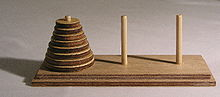
\includegraphics[width=0.57\textwidth]{figures/220px-Tower_of_Hanoi.jpeg}
\end{center}
\caption{Configurazione iniziale del puzzle.}
\end{figure}

Ci sono tre pioli ('A','B' e 'C') su cui trovano collocazione $n$ dischi, numerati da $1$ ad $n$, come presi dal più piccolo al più grande. Le configurazioni valide sono quelle in cui nessun disco si trova collocato sopra un disco più piccolo.
Viene richiesto di portarsi dalla configurazione in cui tutti i dischi risiedono sul piolo 'A' (detta \it{configurazione iniziale}) alla \it{configurazione finale} in cui tutti i dischi sono in 'B', spostando sempre un solo disco alla volta (mossa) e visitando solo configurazioni valide.
\'E nota l'elegante soluzione ricorsiva che risolve il puzzle classico (Édouard Lucas, 1883) col minimo numero di mosse. La soluzione ottima è di fatto unica anche se trova diverse descrizioni/rappresentazioni/interpretazioni in forma iterativa.

Anche nella nostra variante la soluzione ottima sarà unica, e le configurazioni valide sono precisamente le stesse. La variante è caratterizzata dal fatto che i pioli $A$, $B$, $C$ vanno pensati come disposti lungo l'orologio, all'ora esatta, ai 20, ed ai 40 rispettivamente.
Ogni mossa sposta un singolo disco in senso orario, sempre rispettando il vincolo di generare configurazioni valide (nessun disco è disposto sopra un disco più piccolo). In pratica, rispetto al puzzle classico, sono proibiti i seguenti tre spostamenti: $A\not \mapsto C$, $B\not \mapsto A$, $C\not \mapsto B$.\\

In alcuni dei subtask la configurazione finale che si chiede di raggiungere non è quella con tutti i dischi sul piolo $B$. Pertanto, ogni istanza fornisce esplicitamente la configurazione valida che dobbiamo ottenere, specificando il piolo su cui deve essere riposto ogni disco.\\ 

In realtà vogliamo valutare diverse competenze. Nei subtask di tipo~$t=1$ ti chiediamo di listare tutte le mosse di una soluzione ottima, che impieghi il minor numero possibile di mosse.
Nei subtask di tipo~$t=0$ ti chiediamo solamente di computare tale numero di mosse, senza doverle generare, ma più velocemente.
Nel primo caso l'approccio ricorsivo è fortemente consigliato anche nella stesura del codice.
Consigliamo di affrontare prima i subtask di tipo~$t=1$,
e di partire concentrandosi sul caso in cui la configurazione finale sia quella con tutti i dischi sul piolo $B$.


\sezionetesto{Input ed Output}

Per la gestione pulita di input ed output consigliamo di utilizzare il template di soluzione fornito tra gli attachmets alla pagina del problema.
Input ed output avvengono da \verb'stdin'
e da \verb'stdout' rispettivamente.
La prima riga dell'input contiene i due numeri $t$ ed $n$, nell'ordine e separati da spazio. Questi indicano il tipo di richiesta (solo contare o proprio listare le mosse) ed in numero di dischi.
La seconda riga contiene una stringa in $\{A,B,C\}^n$, il cui $i$-esimo carattere specifica il piolo del disco~$i$ nella configurazione finale.
Nel caso in cui $t=0$, il vostro programma deve restituire su \verb'stdout' un unico numero naturale: il minimo numero di mosse che è necessario spendere per portare tutti i dischi sul piolo 'B'.
(Ricodiamo che la configurazione iniziale vede gli $n$ dischi tutti impilati sul piolo 'A', ordinati per etichetta.
Altrimenti, nel caso in cui $t= 1$,
allora il vostro programma deve riportare su \verb'stdout'
la più breve sequenza di mosse che consente di portare tutti i dischi sul piolo 'B', come più precisamente illustrato negli esempi. 


% Esempi
\sezionetesto{Esempio di input/output}

In attachment alla pagina del problema trovate diverse copie input/output tra cui le seguenti.


\vspace{0.5cm}
\esempio{0 3
  
BBB}{15}

\vspace{0.5cm}
\esempio{1 3
  
BBB
}{sposta il disco 1 dal peg A al peg B

sposta il disco 1 dal peg B al peg C

sposta il disco 2 dal peg A al peg B

sposta il disco 1 dal peg C al peg A

sposta il disco 2 dal peg B al peg C

sposta il disco 1 dal peg A al peg B

sposta il disco 1 dal peg B al peg C

sposta il disco 3 dal peg A al peg B

sposta il disco 1 dal peg C al peg A

sposta il disco 1 dal peg A al peg B

sposta il disco 2 dal peg C al peg A

sposta il disco 1 dal peg B al peg C

sposta il disco 2 dal peg A al peg B

sposta il disco 1 dal peg C al peg A

sposta il disco 1 dal peg A al peg B
}

% Assunzioni
%\sezionetesto{Assunzioni e note}
%\begin{itemize}[nolistsep, noitemsep]
%  \item $1 \le n \le 100\,000$.
%\end{itemize}
  
\section*{Subtask}

  \begin{itemize}
    \item \textbf{Subtask 1 [0 punti]:} i casi di esempio forniti alla pagina del problema, essi includono i due casi sopra.
    \item \textbf{Subtask 2 [20 punti]:} $t=1$, $n \le 7$, la configurazione finale è $B^n$.
    \item \textbf{Subtask 3 [20 punti]:} $t=1$, $n \le 10$, la configurazione finale è $B^n$.
    \item \textbf{Subtask 4 [20 punti]:} $t=1$, $n \le 10\,000$, le mosse necessarie sono al più $100\,000$.
    \item \textbf{Subtask 5 [10 punti]:} $t=0$, $n \le 10$, la configurazione finale è $B^n$.
    \item \textbf{Subtask 6 [10 punti]:} $t=0$, $n \le 10$.
    \item \textbf{Subtask 7 [10 punti]:} $t=0$, $n \le 10\,000$, le mosse necessarie sono al più $1\,000\,000$.
    \item \textbf{Subtask 8 [10 punti]:} $t=0$, $n \le 10\,000$, le mosse necessarie sono al più $10\,000\,000\,000$.
  \end{itemize}
  


\end{document}
